\section{Centralized approach}
Consider a set of $m$ PEVs (each with its own specifications) and a MPC prediction horizon of $N = t_f - t_0 + 1$ time steps of duration equal to $T$. The centralized approach consists in computing the optimal charging/discharging schedule for each PEV $p$ at each time step over the prediction horizon, meeting the preferences of the PEV drivers regarding charging time and final state of charge. It is crucial to ensure that the combined power drawn adheres to specified limits and follows a designated pattern, usually calculated to optimize the influence of recharging activities on the electrical grid.
Figure \ref{fig:cen_scheme} shows the block scheme of the centralized approach.
\begin{figure}[H]
    \centering
    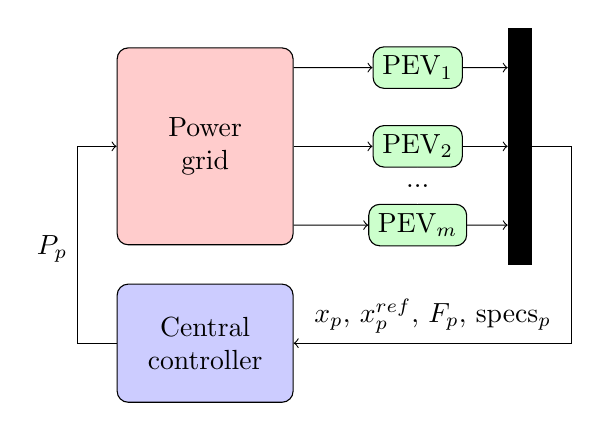
\begin{tikzpicture}[node distance=1.5cm]
        \node (grid) [draw, rectangle, text width=2cm, minimum height=2.5cm, align=center, fill=red!20, rounded corners] {Power \\grid};

        \node (pev2) [draw, rectangle, right of=grid, xshift=1.2cm, fill=green!20, rounded corners] {PEV$_2$};
        \node (pev1) [draw, rectangle, above of=pev2, yshift=-0.5cm, fill=green!20, rounded corners] {PEV$_1$};
        \node (pevm) [draw, rectangle, below of=pev2, yshift=0.5cm, fill=green!20, rounded corners] {PEV$_m$};

        \node (demux) [draw, rectangle, minimum width=0.3cm, minimum height=3cm, fill=black, right of=pev2, xshift=-0.2cm] {};

        \node (cc) [draw, rectangle, text width=2cm, minimum height=1.5cm, below of=grid, align=center, yshift=-1cm, fill=blue!20, rounded corners] {Central \\controller};

        \draw [->] ([yshift=1cm]grid.east) -- node[above] {\Lightning} (pev1.west);
        \draw [->] (grid.east) -- node[above] {\Lightning} (pev2.west);
        \draw [->] ([yshift=-1cm]grid.east) -- node[above] {\Lightning} (pevm.west);

        \draw [->] (pev1.east) -- ([yshift=1cm]demux.west);
        \draw [->] (pev2.east) -- (demux.west);
        \draw [->] (pevm.east) -- ([yshift=-1cm]demux.west);

        \draw [draw=white] (pev2) -- node[midway] {...} (pevm);

        \draw [->] (demux.east) -| ([xshift=0.5cm]demux.east) |- node[pos=0.75, above] {$x_p$, $x^{ref}_p$, $F_p$, specs$_p$} (cc.east);
        \draw [->] (cc.west) -| node[pos=0.74, left] {$P_p$}([xshift=-0.5cm]grid.west) -- (grid);
    \end{tikzpicture}
    \caption{Centralized approach block scheme.}
    \label{fig:cen_scheme}
\end{figure}
\subsection{Problem formulation}
\textbf{Goal}: compute the optimal charging/discharging schedule for a set of $m$ PEVs connected to the power grid.
\\\textbf{PEV charging constraints}
\begin{gather}
    -P^{dis,max}_p \leq P_{p,i} \leq P^{ch,max}_p, \quad \forall p,i \label{constr:c1}\\
    P_{p,i} = P^{ch}_{p,i}-P^{dis}_{p,i}, \quad \forall p,i \\
    \delta^{ch}_{p,i} P^{ch,min}_p \leq P^{ch}_{p,i} \leq \delta^{ch}_{p,i} P^{ch,max}_p, \quad \forall p,i \\
    \delta^{dis}_{p,i} P^{dis,min}_p \leq P^{dis}_{p,i} \leq \delta^{dis}_{p,i} P^{dis,max}_p, \quad \forall p,i \\
    \delta^{dis}_{p,i} + \delta^{ch}_{p,i} \leq 1, \quad \forall p,i \label{constr:c5}
\end{gather}
\\\textbf{Aggregated power constraints}
\begin{gather}
    P_i = \sum_{p=1}^m P_{p,i}, \quad \forall i \\
    P_i \leq P^{max}_i, \quad \forall i \label{constr:c7}
\end{gather}
\\\textbf{PEV state of charge evolution}\\
$\forall p,i:$
\begin{align}
    \begin{cases}
        x_{p,i+1} = x_{p,i} + T (\eta^{ch}_p P^{ch}_{p,i} - \frac{1}{\eta^{dis}_p} P^{dis}_{p,i}) \label{constr:c8}\\
        x_{p,t_0} = (x_0)_p
    \end{cases}
\end{align}
\\\textbf{PEV state of charge constraints}
\begin{gather}
    x_{p, F_p} = x^{ref}_p, \quad \forall p \\
    x^{min}_p \leq x_{p,i} \leq x^{max}_p, \quad \forall p,i \label{constr:c10}
\end{gather}
\\\textbf{Objective function to minimize} \\
\begin{align}
    V = \sum_{i=1}^{N} |P_i - P^{ref}_i|
\end{align}
that is possible to linearize, introducing the auxiliary variables $t_i$:
\begin{gather}
    V = \sum_{i=1}^{N} t_i \\
    s.t. \quad -t_i \leq P_i - P^{ref}_i \leq t_i, \quad \forall i \label{constr:c13}
\end{gather}
We then introduce a small perturbation term $\xi_{p,i}, \forall p,i$ in $V$ weighting the power to satisfy Assumption 2.4 of \autocite{VUJANIC2016144}. The final form of the objective function is the following:
\begin{align}
    V = \sum_{i=1}^{N} (t_i + \sum_{p=1}^m P_{p,i} \xi_{p,i}) \label{constr:c14}
\end{align}
\textbf{Charging/discharging schedule} \\
At each iteration of the MPC, the optimal control schedule is computed by solving
\begin{align}
    \begin{bmatrix}
        P^{ch}\\
        P^{dis} 
    \end{bmatrix}
    = \argmin_{P^{ch}, P^{dis}} V
\end{align}
subject to the constraints (\ref{constr:c1})-(\ref{constr:c10}), (\ref{constr:c13}), (\ref{constr:c14}),
\\and using the following notation:
$$P^{ch/dis} \triangleq \begin{bmatrix} 
    P^{ch/dis}_{1,1} & \dots & P^{ch/dis}_{1, N} \\
    \vdots & \ddots & \vdots \\
    P^{ch/dis}_{m,1} & \dots & P^{ch/dis}_{m, N}
\end{bmatrix}$$ 
The charging/discharging schedule of each PEV is:
$$P_p = \begin{bmatrix} P_{p,1} & \dots & P_{p, N} \end{bmatrix}^T = (P^{ch}_{p}-P^{dis}_{p})^T.$$
\subsection{Solution algorithm}
\begin{algorithm}[H]
    \caption{Centralized algorithm.}
    \label{algo:cen}
    \SetKwInOut{Input}{Input}
    \SetKwInOut{Output}{Output}

    \Input{$\Big\{N, T, m, (P^{max}_i, P^{ref}_i)_{i=1}^N, (P^{ch,max}_p,$
    $ P^{ch,min}_p, P^{dis,max}_p, P^{dis,min}_p, \eta^{ch}_p, \eta^{dis}_p,$
    $(x_0)_p, x^{max}_p, x^{min}_p, x^{ref}_p, F_p)_{p=1}^m,$ 
    $(\xi_{p,i})_{i,p=1}^{N,m}\Big\}$}
    \Output{$\Big\{(P^{ch}_{p,i}, P^{dis}_{p,i})_{i,p=1}^{N,m}\Big\}$}
    
    \BlankLine
    \tcp{Solve the optimization problem}
    \vspace*{-0.4cm}
    $$\begin{bmatrix}
            P^{ch}\\
            P^{dis} 
        \end{bmatrix}
        = \argmin_{P^{ch}, P^{dis}} \sum_{i=1}^{N} (t_i + \sum_{p=1}^m P_{p,i} \xi_{p,i}) $$
        $$s.t. \quad (\ref{constr:c1})-(\ref{constr:c10}), (\ref{constr:c13}), (\ref{constr:c14})$$
\end{algorithm}
    \noindent Notice the large quantity of variables and constraints that the central controller has to deal with. 